
\documentclass{sig-alternate-05-2015}

\begin{document}

\title{ Roommate Finder Web Application}


\numberofauthors{4}

\author{
% 1st. author
\alignauthor
Riken Shah\\
       \affaddr {NC State University}\\
       \affaddr{Raleigh, North Carolina}\\
       \department{Computer Science}\\
       \email{rshah9@ncsu.edu}
% 2nd. author
\alignauthor
Mateenrehan Shaikh\\
        \affaddr {NC State University}\\
       \affaddr{Raleigh, North Carolina}\\
       \department{Computer Science}\\
       \email{mshaikh@ncsu.edu}
% 3rd. author
\alignauthor Aaroh Gala\\
\affaddr {NC State University}\\
       \affaddr{Raleigh, North Carolina}\\
       \department{Computer Science}\\
       \email{agala@ncsu.edu}
\and
% 4th. author
\hspace{1cm}
       \alignauthor Himani\\
       \affaddr {NC State University}\\
       \affaddr{Raleigh, North Carolina}\\
       \department{Computer Science}\\
       \email{hhimani@ncsu.edu}
\and       
}
\sloppy


\maketitle
\begin{abstract}
In a particular semester around 34000 students study at North Carolina State University. Along with studies comes the stress of looking for roommates who are compatible with most of their preferences. In most of the cases, students end up selecting a house, however, the search for a roommate is inefficient. In this work, we have surveyed and examined the problems of communication gap and trust issues faced by current graduate students despite having social media groups to bond with each other for finding potential roommates. We look into the existing solutions developed and analyze the code as well as results in great details and propose an improved solution to solve this problem. We also demonstrate the inefficiencies of existing solutions and how we can modify those to improve the overall results. At the same time, we also propose radically different attributes and features that will help in making the application more dynamic, scalable, feature-rich and user-friendly.
\end{abstract}

\keywords{Roommate Rapport Scale (RRS),recommendation system, in-built chat, Machine Learning, Graph mining}

\section{Introduction}

The main goal of software engineering is to solve real-world problems using efficient use of technology. There are very few applications that focus on some of the pertinent problems like finding a roommate who is compatible. This paper focuses on the solved problem of finding compatible roommates for incoming non-resident NC State students. Our goal is to derive meaningful results from the survey conducted, browse through relevant journals, and develop a robust, user-friendly, and scalable web application to solve the problem. Our survey strongly emphasized the need for a separate web application for roommate finding. Though there are several social media platforms such as Facebook or WhatsApp that allow people to create 'roommate finder' groups, posts accumulate one after another and reading through all the posts becomes almost impossible. Also, we try to find the pros and cons of the existing application by detailed analysis and research about its code structure and outcomes. Drawing conclusions from the survey results, we infer that poor roommate finding methods necessitate a user-friendly, reliable web application that attests a user as a good roommate through the virtue of recommendations.

In the further sections we dive deeper into various modules of an existing project and how are we planning to improve it. We also propose some new features which would make the application more intuitive and efficient. We look at various code smells that are introduced in the existing code base and our plans on how to eliminate those. We also plan to maintain a continuous development and continuous integration pipeline for our project following the agile methodologies making sure that we provide small deliverable every iteration. We plan to conduct regular meetings to decide on our deliverables as well.

The rest of the paper is distributed as follows. We talk about literature in this domain in Section 2, including the background and motivation of such work. Section 3 talks about problems with existing system. Then in Section 4, we talk about various code smells that we discovered in existing code base. Enhancements and Implementation is detailed in Section 5. We propose the use cases of the system in Section 6. Section 7 details the architectural components of the project. We conclude in Section 8 with future scope in section 9. 

\section{Literature Review}
Before delving into building the application, we did a careful analysis of existing systems. We read a few research papers and it was evident that interpersonal compatibility, food preferences and sharing the living space with someone with similar personality is a more satisfying experience. A literature review of roommate understanding and preferences depicted that the RRS(Roommate rapport scale) discriminated between those who selected their roommates and those whose did not. Naturally, those who choose their roommates have better rapport. If a student makes good friends with his roommates, it would have a positive impact on his psychological well-being, personal growth, purpose in life, and self-acceptance. Evidence also suggests that women and culturally similar pairs were higher on both trust and intimacy [1]. \\


A student with a roommate conflict due to difficulty communicating with the roommate or advocating for their needs may have a negative impact on their academics [3]. Studies suggest that happiness and depression may be highly contagious across social ties [4]. This means an incompatible roommate could be a potential cause for unhappiness and could be detrimental to the social circle. Most students who live with roommates for the first time often find it difficult to communicate and adjust with their roommates. So, it is essential for the student to pair up with like-minded people as their roommate [6].\\

Students often do not choose roommates and may experience personality mismatches. In a sample of 31,500 students in a nationwide survey, 50.1\% of women and 44.1\% of men reported frequent or occasional conflict with roommates or housemates [2]. In a nationwide survey, 5.6\% of students reported that roommate difficulties hindered their academic performance. Roommate conflict is a widespread experience among college students.\\

A customized application for NC State students would help overcome the disadvantages of traditional roommate finder applications. In order to ensure optimal matching, our system provides the option of priorities to individual preferences at the users end. Based on the priority matching we enable the users to find a satisfactory match as a roommate. If the priority is high, the preferences must strictly match, conversely the preferences with low priority may or may not match. Another issue with such roommate finder applications is reliability. The user could be a fraudster and may not be someone he claims to be. This calls into question the reliability of the application and compromises the safety of other users interacting with the fraudster. 
\\
\subsection{BACKGROUND AND MOTIVATION}

There are many research papers which show how interpersonal compatibility, food preferences and other attributes contribute towards satisfaction of sharing the living space with someone who has a personality similar to theirs. A literature review of roommate understanding and preferences depicted that the RRS discriminated between those who selected their roommates and those who did not. If a student makes good friends with his roommates, it would have a positive impact on his psychological well-being, personal growth, purpose in life and self-acceptance [1]. 
\\

\begin{figure}[h]
\centering
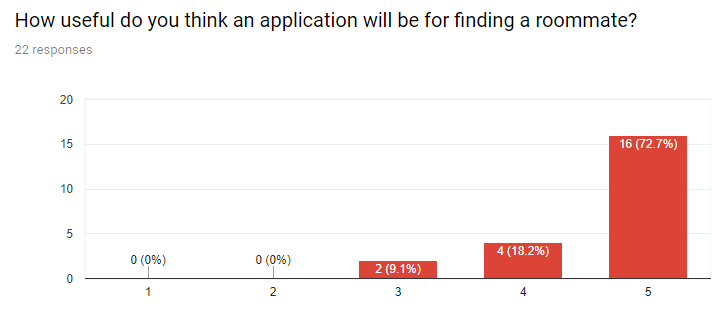
\includegraphics[width=8.5cm]{1.png}\\
\caption{Importance of Application}
\end{figure}
\\
From the survey of requirement of an application to find a roommate, we found out that most of the user told that a different application for this is needed. Hardly any user denied with the necessity of a different application to find roommate. The survey results are presented in figure 1.
\\
\begin{figure}[h]
\centering
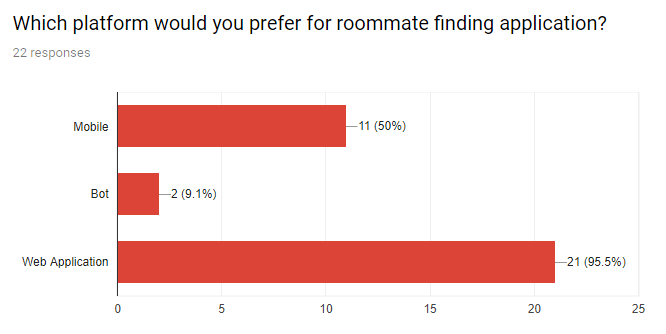
\includegraphics[width=8.5cm]{2.PNG}\\
\caption{Preferred Platform}
\end{figure}
\\
Even though mobile devices are widely used and preferred for everything. But people preferred a web application for finding a roommate over mobile devices. This can be for many reasons like they can multitasking of looking social media, online search etc simultaneously. The survey results are presented in figure 2.
\\
\begin{figure}[h]
\centering
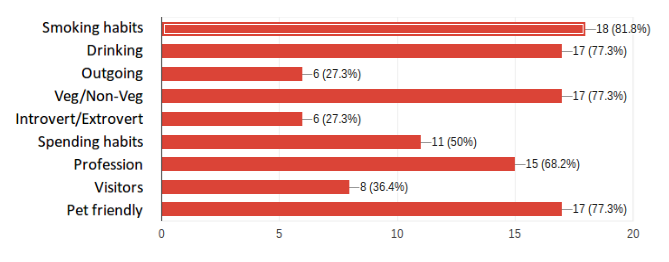
\includegraphics[width=8.5cm]{3.PNG}\\
\caption{Important Attributes}
\end{figure}
\\
From Survey result shown in Figure 3, we can see a list of attributes which are important or consider with high importance while looking for roommates. We can also see that there is a similarity or few clusters of attributes considered as important by most of the user.
\\
\begin{figure}[h]
\centering
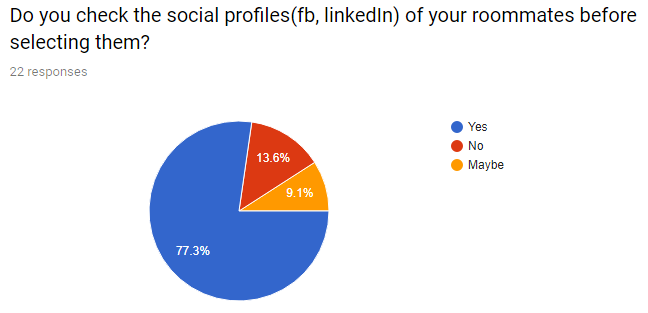
\includegraphics[width=8.5cm]{5.PNG}\\
\caption{Social Media}
\end{figure}
\\
From the survey, we found out that most of the users look at the social media profile of other person while finding roommates. This can be found in Figure 4.
\\
\begin{figure}[h]
\centering
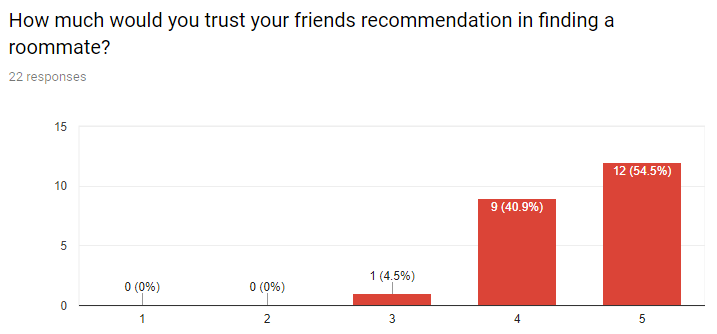
\includegraphics[width=8.5cm]{6.PNG}\\
\caption{Friend Recommendation}
\end{figure}
\\
We asked user how important do they consider friends recommendation while choosing roommates and we found out that most of the user will highly consider a friends recommendation while choosing a roommate. This can be found in Figure 5.

We also asked other question like which attributes do you think apart from the given are more important while choosing roommate and hardly people responded. Because for most of the user a common cluster of attributes were more important.


\section{Problems with Existing System}

Before getting started, we analyzed the current Roommate Finder web application and we found a couple of problems with the existing system. 
\begin{enumerate}
\item \textbf{Incoherent results -}When a user sets up a profile in the web application, clicking on the profile icon sometimes showed profile of a different user. In the little time that we worked with the existing system, we were not able to figure out the cause of the problem but this was a major bug.
\item \textbf{Broken functionalities -}Search was not working for some users, it was giving application errors in case user does not set up their profile information with all the essential details and in an improper format.
\item \textbf{Email Verification ambiguities -}The system worked on email verification but at times, we were able to login without completing the email verification. The email verification to validate a user was done using a personal email id, so we decided to change that to a more standard and platform specific email id. A standard email id helps establish trust in the application as compared to a personal email id.
\item \textbf{Database Design -}There was only one table in the database which stored user information and their profile. All the information was clubbed and stored in one table, even though normalization is good but we intend to work on roommate recommendation and implement back-end algorithms to come up with sound roommate suggestions so we would need to denormalize some data and seriously thinking about database design to meet our goals.
\item \textbf{No Modularity -}Modularity was introduced in the project structure but it was not adhered to, most of the code was put into one file.
\end{enumerate}


\section{Code Smells}
For detecting the code smells we used the paper ``Do they really smell bad" where all the parameters were given for evaluation of code smell.[10]
\begin{enumerate}
\item \textbf{Duplicate code -} In the existing code-base there were quite a few places where there was duplicate code. For example, the model/users.js and model/request.js was exactly the same as app/model/users.js and app/model/request.js.
\item \textbf{Data should be private -} In the app.js we found that the mongo URL with the database username and password was available. Anyone can potentially delete the database with just one command. In routes/index.js the Gmail credentials were in clear of the user who authenticated the SMTP server. A good practice would be to have them included in the .env file so that the credentials are not public on GitHub.
\item \textbf{Spaghetti Code -} There were many methods without structure. The app/views/ had many files without structure.
\item \textbf{Long Methods -} The routes/index.js had some very long methods which could have easily been broken down into small methods. For example, the database update method could have been included in the model/user.js instead of exporting the users.js and then updating it routes files. The routes file should have been way simpler just showing the routes each request will take.
\item \textbf{Lazy Class -} There were a few lazy classes as well which were not doing much in the code. The app/views/login had 2 files with just one line of code which could have been easily merged. 
\item \textbf{Testing -} Testing of the code is not done at all. So we cannot verify the correctness of the search algorithm.
\end{enumerate}\\

\section{Enhancements and Implementation}
Because of the reasons stated above, we decided to go ahead with making a new system from scratch, we plan to build a modular code because it helps not only in development but also debugging and testing application. In modularity, we plan to follow MVC architecture where we are going to divide our project structure in three layers-one for interaction with database, one for the back-end business logic and one for interaction with the user. 
\\

As per technical stack, we will build the web application in Node.js because it is scalable, fast and robust, the front end will be in HTML/CSS and bootstrap. Also, we plan to use an existing robust library i.e. passport.js for user authentication and authorization. We will create a standard email id for handling the email verification process. We will be using MongoDB for database design and handling user data. We understand that roommate recommendation is a keynote feature of our application and we planning to use Graph mining algorithms to come up with relevant recommendations. Along with building a robust application with standard features we are planning to integrate some amazing cool features like in built chat and roommates recommendation, which are discussed in detail in section 6.\\

Here is a comparison chart of our system with the existing application.
\begin{table}[h]
\centering
\caption{Comparing with the existing system}
\begin{tabular}{|c|c|c|l|} \hline
Metrix&Original System&Proposed System\\ \hline
Recommendation &- -&++\\ \hline
Search &-&++\\ \hline
Security &- -&++\\ \hline
Speed &++&+\\ \hline
\end{tabular}
\end{table}

\subsubsection{Recommendation}
The current system did not have any recommendation system where the roommates would be recommended based on their preferences. We will be using machine learning to recommend the roommates. 
\subsubsection{Search}
The current system does the searching by just a database query based on the certain selection. If they search cannot match any one of the parameters given parameters than it will not show any results. Our system will implement a better search algorithm with more parameters and suggest the users the closest roommates.
\subsubsection{Security}
Our proposed system will enhance the security as we will be using the standard practices like not exposing credentials on public repositories like Github, using standard tested libraries rather than reinventing the wheel which can consist of bugs. The original system did not follow this standard practices and they had the credentials in clear text on Github and they tried to create the authentication system (which had bugs) when there are many libraries available which are doing the same things in a better way.  
\subsubsection{Speed}
The speed of our application will be slightly slower than the current system as we will be using the machine learning to recommend the roommates but since the feature is very useful users would prefer a slightly slower system which can recommend them, roommates.


\section{USE CASES}
After thorough analysis and conducting a survey on the application we found out that there are few additional functionality which can be added to enhance the application and make it more user friendly. After survey and brainstorming we found there is a necessity for three major additional use cases required in the system. They are:
\begin{enumerate}
\item \textbf{Chat Option}:
Roommate finder helps in finding roommates on the application based on the attributes and the search query. But only finding a roommate may not be a good idea unless there is an option of chatting with the other person whom you think would be a good roommate for you. There can be two ways to connect the user. External and internal. For external communication, we need to use other platform or social media. The user is being forced to share personal details like email id, phone number or social media account. This might be uncomfortable for many user. Also, this can lead to privacy issues, where users data can be fetch and used for some other purpose without users concern. In internal communication, we can create an inbuilt chat application, where two users can communicate with each other without sharing any personal information like email id, phone number or social media profile. Looking at the drawbacks of the external communication system which can be easily tackled by internal communication system. We plan to implement an internal chat application, where once the user find a roommate. The user has an option to start a chat with the user, and the other user will be notified that some person wants to communicate with you or has initiated a communication on the application. Since, the chat option is inbuilt chatbox. User details would not be reviled and only user name will be displayed. This makes the communication more secured.
\item \textbf{Machine Learning}
Now a days, every search is made more efficient by using machine learning algorithms. Finding a roommate can also be considered as an search query based on few parameters like preferences, etc. Running a simple query and returning a list of user which can be potential roommates increases the task of the user. The user needs to look at all the profile and see for more similarities between him/her and the list of people. But this can be reduced by using machine learning algorithms. The machine learning algorithms will be trained in such a wait that rather than returning a simple list of users which satisfies the parameters, it can give list of users in an order which are more similar or has more attributes similar to the search user. In simple terms, machine learning algorithms can return a list of user which satisfy the attributes in such a way that the possibility of two people gelling up together is maximum at top to minimum at the end. We plan to implement machine learning algorithms to make the search better which will help the users to find roommates which have more similarities and the likeliness to gel up well together.
\item \textbf{Recommendation}
Searching roommates based on a list of few attributes might or might not result in finding a perfect roommate. Roommates get along well together if they have similar personalities or something in common. For E.g. if two person like football, then there are more chances of them getting along together than two people of which one like football and other does not like football. This could be more better if both the roommates like the same football team. Knowing the personality of a person can help in finding a better roommate then a normal search query which gives list of user which satisfy some criteria. We are planning to implement and include a feature which analysis the user personality based on social media account. Once the personality, likes, dislikes are known. We can use machine learning algorithms to make better predication and recommendation of roommate while choosing a roommate.
\end{enumerate}

\section{ARCHITECTURE}
\begin{figure}[h]
 \centering
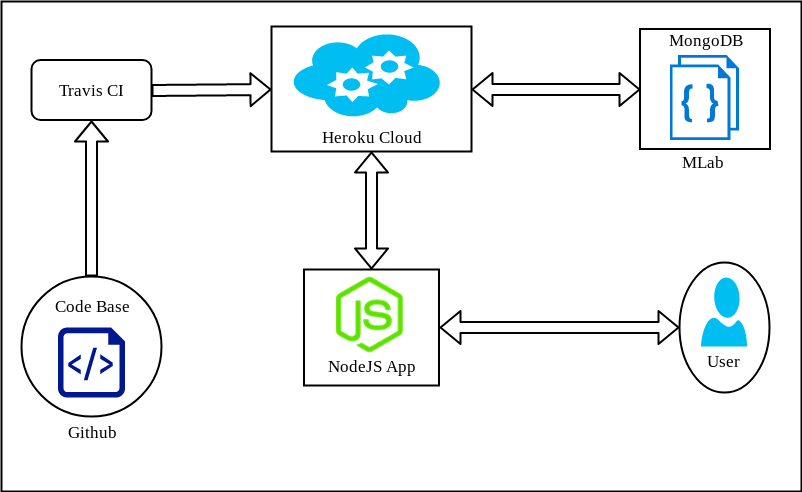
\includegraphics[width=8.5cm]{ArchitectureRoomate.png}\\
\caption{Use case diagram of the application}
\end{figure}

Figure 2 shows the proposed architecture of the application. We take into account various modules that are present in the system and also how they communicate with one another. \\

The master branch of the GitHub repository is integration with Travis continuous integration pipeline so that any changes that we push to the master branch will be automatically built on Travis and all the test cases will be run. If both the build and test cases passes then the code is pushed on the Heroku server where the NodeJS app resides. The web server will have UI Components, Application Logic, Security and Data unit. The application logic will includes authentication, registration and searching. The database used for the application is  MongoDB at MLab Sandbox Database-as-a-Service. 

\section{FUTURE SCOPE}

\begin{enumerate}
\item \textbf{Mobile Support-} From our survey analysis we found that there were many users who wanted the application on their mobile devices like android and IOS. So providing a mobile application will enhance user experience and provide ease of use. \\

\item \textbf{Search House-} Once the roommate is found both the roommates can even search for a location where they want to rent or buy a house. This will make our application more useful now not only can they find roommates but they can search houses together.\\

\item \textbf{Combined Roommate Search-} After two people have agreed to be roommates of each other, they both can search other roommates as a combined user. In such cases, preferences of both the users can be taken into consideration to find the potential match. Additionally, group chat feature could also be introduced for a user to communicate multiple people who may be planning to stay together.\\

\item \textbf{Review Roommates-} A user can review his roommate on a web application. This review can be anonymous or identified. Such reviews can be useful for other users to make better-informed decisions.\\
\end{enumerate}

\section{CONCLUSION}
After having established that sharing living space with a person with similar interests and preferences is more satisfactory and healthy in general, our application plans to incorporate crude elementary details and preferences which make roommates compatible. We are planning to build a robust Recommendation system using Machine learning algorithm.We are planning to mine relevant data-sets for our application from the widespread use of social media. Having relevant data-set from the users would help us better understand if our recommendation results offer good roommate matching and it is persistent to the actual experience of our target audience. Having the accurate data-set will help us revisit and improve the metrics. Also, an online chat application will help the user in connecting more efficiently while choosing a roommate.\\

\begin{thebibliography}{9}
\bibitem{1}Erb, S.E.,Renshaw, K.D.,Short, J. L., Pollard, J. W. (2014),
The importance of college roommate relationships: A review and systemic conceptualization, Journal of Student Affairs Research and Practice.
\bibitem{2}M. Shekhawat, S. Deshmukh, G. Monroy, A. Tiwari, X. He, H. Shin, Y. Hong and H. Lu, Usability Test of Personality Type within a Roommate Matching. Journal of International Technology and Information
Management, Volume 25 | Issue 1\\
\bibitem{3}Ashley M. Payne, The challenges of living with a roommate: the
impact on students with disabilities' residential
experience, Rowan University\\
\bibitem{4}Ezra Golberstein, Janis L. Whitlock, and Marilyn F. Downs, Social contagion of mental health: Evidence from college roommates, Health Econ. 2013 Aug; 22(8): 965-986\\
\bibitem{5}https://yocket.in\\
\bibitem{6}Kimberly Halpin, Roommate Rants: Understanding Roommate
Conflicts among MSU Students, Journal of Undergraduate Research
at Minnesota State University, Mankato. Volume 9 | Article 3\\
\bibitem{7}https://github.com/googlemaps/google-maps-services-js\\
\bibitem{8}https://www.mongodb.com/blog/post/the-modern-application-stack-part-2-using-mongodb-with-nodejs\\
\bibitem{9}Itti Hooda, Rajendra Singh Chhillar,"Software Test Process, Testing Types and Techniques", International Journal of Computer Applications (0975 - 8887) Volume 111 - No 13, February 2015.\\
\bibitem{10}Fabio Palomba, Gabriele Bavota, Massimiliano Di Penta, Rocco Oliveto, Andrea De Lucia (2014),
Do they Really Smell Bad? A Study on Developer's
Perception of Bad Code Smells\\
\end{thebibliography}
\end{document}
